%%%%%%%%%%%%%%%%%%%%%%%%%%%%%%%%%%%%%%%%%%%%%%%%%%%%%%%%%%%%%
%%	Constitutive model form									%
%%%%%%%%%%%%%%%%%%%%%%%%%%%%%%%%%%%%%%%%%%%%%%%%%%%%%%%%%%%%%

\section{Effective constitutive model formulation}

%-----------------------------------------------------------
%	Kinematics
%-----------------------------------------------------------
\subsection{Kinematic considerations}
	
	To formulate any soft tissue constitutive model, the choice for kinematic basis is the first step. The choice of kinematic basis has significant impact on the constitutive model form, model parameter covariance, number of parameters necessary and even the quality of fit for parameter estimation. There are two categories for selecting the kinematic basis. 
\begin{enumerate}
\item Invariants
\item Finite deformation strain tensors
\end{enumerate}

\subsubsection{Invariants} \label{sec:invariants}
%-------	Possible invariants	-------%
	Using invariants is a common choice, which are scalar functions of the right or left Cauchy Green tensor which are independent of rigid body motion. Each invariant describes a facet of deformation: isotropic, volumetric strain, anisotropic, or interactions between them. The breadth of choices, allows for more freedom in selecting a combination of invariants for constitutive models that best describes the mechanisms in the tissue. The three isotropic invariants of the right Cauchy Green tensor are $I_1 = Tr(\mathbf{C})$, $I_2 = \frac{1}{2}\left( Tr(\mathbf{C})^2 - Tr(\mathbf{C}^2)\right)$, $I_3 = \det(\mathbf{C})$. The extension for anisotropic materials is summarized by Holzapfel \cite{holzapfel_nonlinear_2000}. The usual starting point is $I_4 = \mathbf{m}\cdot \mathbf{C} \mathbf{m}$, where $\mathbf{m}$ is a unit vector for material axis, or the preferred direction, most commonly that of the constituent fibers, such as collagen and elastin. Other pseudo invariants include $I_5 = \mathbf{m}\cdot \mathbf{C}^2 \mathbf{m}$, $I_6$ and $I_7$ which are equivalent of $I_4$ and $I_5$ for another family of fibers along some $\mathbf{n}$, $I_8 = \mathbf{m}\cdot\mathbf{C}\mathbf{n}$ and $I_9 = (\mathbf{m}\cdot\mathbf{n})^2$ can be used to describe the interaction between these two fiber families \cite{sacks_novel_2016}\cite{avazmohammadi_novel_2017}, etc. Optimal choice for the invariants can help with parameter estimation by reducing the number of parameters needed. 


%-------	Why traditional invariants are not suitable	-------%	
	However, the use of invariants do not lend itself to creating a single generalized form. For example, there is no specific set of invariants and pseudo invariants that can cover all forms of material behavior of interactions. Including all such invariants, will only lead to an unmanageable number of parameters. One example is when modeling the effects of fiber rotation in tissues with widely distributed fiber orientations. This is one of the most difficult behavior to model using phenomenological approaches. Fiber rotation manifests as coupling interactions between axial stretches in the mechanical response of soft tissues. Invariant based models cannot easily reproduce this effect. One approach is to use the Driessen model \cite{driessen_structural_2005}, where additional fiber families are added until it can match the response of the soft tissue. However, this significantly increases computational costs and requires two additional parameters for each additional fiber family. The number of fiber families needed and their orientations also cannot be generalized. Further extensions to this approach is to incorporate the fiber orientation distribution directly, such as in meso-scale structural approaches \cite{sacks_incorporation_2003a, fata_insights_2014, zhang_meso_2016}. However, this also increases the complexity and computational cost of the model, which defeats the point of phenomenological approaches entirely. Adding coupling invariants such as $I_8$ and $I_9$ are also an option. However, the inherent similarities between these invariants makes it difficult to incorporate them all in a generalized constitutive model form. 
    
    
    
\subsubsection{Conventional finite deformation strain tensors} \label{sec:straintensor}

	The components of strain tensors, such as the Green-Lagrange, $\mathbf{E}$, right Cauchy-Green, $\mathbf{C}$, left Cauchy-Green, $\mathbf{B}$, or the right stretch, $\mathbf{U}$ can be used directly in the constitutive model. One example using strain tensor components is the commonly used generalized Fung model \cite{fung_biomechanics_1993}. The effects of choice of strain tensor is not entirely clearly. Specifically, $\mathbf{U}$ scales linear with the deformation, whereas $\mathbf{E}$, $\mathbf{C}$, and $\mathbf{B}$ scales quadratically with the deformation. Functionally, these tensors behave very similarly. For example, $\mathbf{E}$ is just $\mathbf{C}$ scaled by $1/2$. More often than not, the choice is to simply default to $\mathbf{E}$, which leads to a simple mathematical form for the stress-strain relationship and the elasticity tensor. Although, it is common to use the componential of $\mathbf{E}$ directly, it can be helpful express them with respect to the material axis, $\left[\mathbf{E}\right]_{\mathbf{m}_0,\mathbf{n}_0}$, so that it is not dependent on the specimen orientation or the coordinate system. That is 
\begin{equation} \label{eqn:greenstrain}
E_m = \mathbf{m}_0\cdot\mathbf{E}\mathbf{m}_0, \quad E_n = \mathbf{n}_0\cdot\mathbf{E}\mathbf{n}_0, \quad E_{\phi} = \mathbf{m}_0\cdot\mathbf{E}\mathbf{n}_0,
\end{equation} 
should be used to formulate the constitutive model.

%-------	Hencky strains		-------%

    One additional strain basis we have considered is the Hencky strains, which is the logarithmic strain calculated from the upper triangular decomposition of the deformation gradient tensor with respect to the material axis as described in Criscione \textit{et al.} \cite{criscione_experimentally_2003a} and then further expanded on by Srinivasa \cite{srinivasa_use_2012} and Freed \cite{freed_logarithmic_2015, freed_conjugate_2017, erel_stress/strain_2017}. This has the following number of advantages: (1) The decomposed strains are easy to interpret physically, (2) it results in an extremely simple mathematical form the Cauchy stress, (3) the logarithmic strains are beneficial when dealing with experimental errors in reference configurations, and (4) It is expected to be slightly less correlated in comparison to the Green Lagrange strains. The Hencky strains have the greatest in difference compared to the Green-Lagrange strains, and are thus a good choice for comparing the strain bases.
    
    
%%%%%%%%%%%%%%%%%%%%%%%%%%%%%%%%%%%%%%%%%%%%%%%%%%%%%%%%%%%%
%-------------------	begin FIGURE 	-------------------%
\begin{figure}
\centering
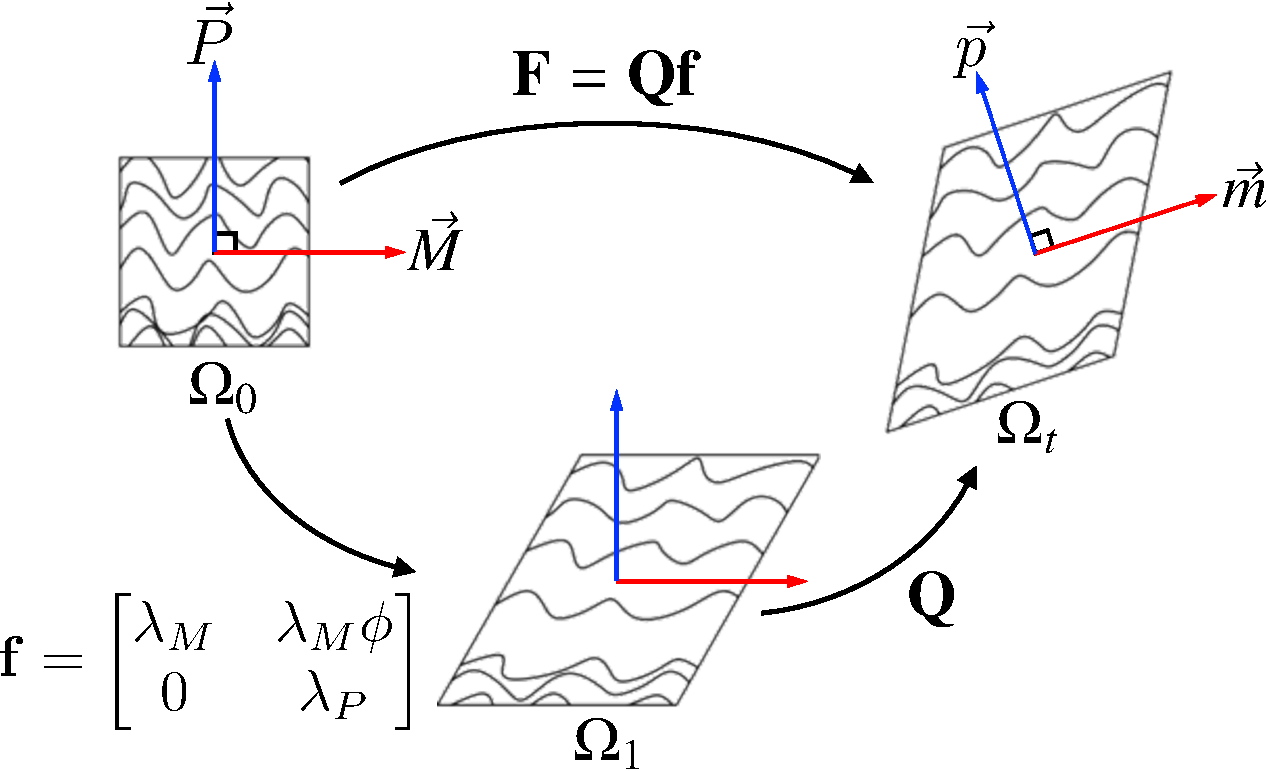
\includegraphics[width=5in]{Figures/henckykinematics}
\caption{The upper triangular decomposition of the deformation gradient tensor with respect the preferred material axis of soft tissues, whose components are used to define the Hencky strains.}
\label{fig:henckykinematics}
\end{figure}
%-------------------	 end FIGURE 	-------------------%
%%%%%%%%%%%%%%%%%%%%%%%%%%%%%%%%%%%%%%%%%%%%%%%%%%%%%%%%%%%%
    
    
    The Hencky strains can be formulated as followed. Briefly, the upper triangular decomposition, $\mathbf{f}$, when expressed with respect to the material axis of the tissue is given by
%==========================================================%
%-------------------	begin EQUATION 	-------------------%
\begin{equation}
\begin{aligned}
\left[\mathbf{f}\right]_{\mathbf{m}_0,\mathbf{n}_0} = \begin{bmatrix}
\lambda_m 	& \lambda_m\phi \\
0			& \lambda_n
\end{bmatrix}.
\end{aligned}\label{eqn:uppertriangulardecomposition}
\end{equation}
%-------------------	 end EQUATION 	-------------------%
%==========================================================%
Here, $\mathbf{m}_0$ is the material axis in the referential configuration, which is generally the preferred direction of the fibers embedded in the tissue, $\mathbf{n}_0$ is the direction perpendicular to $\mathbf{m}_0$, $\mathbf{m}_t$ is the material axis in the deformed configuration, $\mathbf{n}_t$ is the direction perpendicular to $\mathbf{m}_t$, $\lambda_m$ and $\lambda_n$ are the stretches along these axes respectively, and $\phi$ is the angle of shear between $\mathbf{m}_0$ and $\mathbf{n}_0$. The corresponding deformation gradient tensor can thus be expressed as 
%==========================================================%
%-------------------	begin EQUATION 	-------------------%
\begin{equation}
\begin{aligned}
\mathbf{F} = \lambda_m\mathbf{m}_t\otimes\mathbf{m}_0 + \lambda_m\phi\mathbf{m}_t\otimes\mathbf{n}_0 + \lambda_n\mathbf{n}_t\otimes\mathbf{n}_0.
\end{aligned}
\end{equation}
%-------------------	 end EQUATION 	-------------------%
%==========================================================%
The Hencky strains ($\gamma_1, \gamma_2, \gamma_3$), which are functions of the components of $\mathbf{f}$, can be determined using, 
%==========================================================%
%-------------------	begin EQUATION 	-------------------%
\begin{subequations}\label{eqn:henckystrains}
\begin{align}
\gamma_1 &= \log(\lambda_m), &	\gamma_2 &= \log(\lambda_n), 	& \gamma_3 &= \phi	\\
\lambda_m &= \mathbf{m}_t\cdot\mathbf{F}\mathbf{m}_0, &	\lambda_n &= \mathbf{n}_t\cdot\mathbf{F}\mathbf{n}_0,	&	\phi &= \left(\mathbf{m}_t\cdot\mathbf{F}\mathbf{m}_0\right)^{-1}\mathbf{m}_t\cdot\mathbf{F}\mathbf{n}_0.
\end{align}
\end{subequations}
%-------------------	 end EQUATION 	-------------------%
%==========================================================%
    
    
%-------	Hencky vs. Green-Lagrange strain	-------%

	We are most interested in the difference between Green-Lagrange and the Hencky strains for the formulation of the effective constitutive model (Summary Table \ref{tb:greenvshencky}). Firstly, as stated above , Hencky strains lead to a very convenient form for the Cauchy stresses,
%==========================================================%
%-------------------	begin EQUATION 	-------------------%
\begin{equation}\label{eqn:cauchystressform}
\mathbf{T}	= \frac{1}{J} \dpd{\Psi}{\gamma_1} \mathbf{m}_t\otimes\mathbf{m}_t 
			+ \frac{1}{J} \dpd{\Psi}{\gamma_2} \mathbf{n}_t\otimes\mathbf{n}_t 
			+ \frac{\lambda_n}{J\lambda_m} \dpd{\Psi}{\gamma_3} \left(\mathbf{m}_t\otimes\mathbf{n}_t + \mathbf{n}_t\otimes\mathbf{m}_t \right).
%\\
%\dpd{\Psi}{\gamma_1} 	= J \mathbf{m}\cdot\mathbf{T}\mathbf{m}, \quad 
%\dpd{\Psi}{\gamma_2} 	= J \mathbf{s}\cdot\mathbf{T}\mathbf{s}, \quad 
%\dpd{\Psi}{\gamma_3} 	= J \frac{\lambda_m}{\lambda_n}\mathbf{m}\cdot\mathbf{T}\mathbf{s}.
\end{equation}
%-------------------	 end EQUATION 	-------------------%
%==========================================================%
where $\Psi$ is the strain energy density function.
In comparison, the 2nd Piola Kirchhoff stress with Green-Lagrange strains is,
%==========================================================%
%-------------------	begin EQUATION 	-------------------%
\begin{equation} \label{eqn:2ndpkstressform}
\mathbf{S} = \dpd{\Psi}{E_m}\mathbf{m}_0\otimes\mathbf{m}_0
+ \dpd{\Psi}{E_n}\mathbf{n}_0\otimes\mathbf{n}_0 
+ \frac{1}{2}\dpd{\Psi}{E_{\phi}}\left(\mathbf{m}_0\otimes\mathbf{n}_0 + \mathbf{n}_0\otimes\mathbf{m}_0\right),
\end{equation}
%-------------------	 end EQUATION 	-------------------%
%==========================================================%
with the Cauchy stress obtained from push forward, $\mathbf{T} = (1/J) \mathbf{F}\mathbf{S}\mathbf{F}^\mathsf{T}$. Expressing the Green-Lagrange strain with respect to the material axis, ${E_m, E_n, E_\phi}$, is preferred, so that the model parameters are invariant with respect to rigid body motion and changes in the reference coordinate system. There isn't a significant advantage to either strain measure here. However, we do note that the partial derivative of Green-Lagrange strain, $\pd{\mathbf{E}}{\mathbf{C}}$ (Eqn. \ref{eqn:partialgreens}), is much simpler than that of the Hencky strains, $\pd{\gamma}{\mathbf{C}}$ (Eqn. \ref{eqn:henckyderivatives}). As a result, the elasticity tensor, $\mathbb{C} = C_{ijkl}$, for the Hencky strain is much more complex (see Appendix \ref{sec:elasticitytensor}). 

	One other aspect is the difference in correlation between model parameters when using Green-Lagrange strain, $\{E_m, E_n, E_\phi\}$ vs. using Hencky strains $\{\gamma_1, \gamma_2, \gamma_3 \}$. For example, using the for form of the generalized Fung model,
%==========================================================%
%-------------------	begin EQUATION 	-------------------%
\begin{subequations} \label{eqn:generalizedfungmodel}
\begin{align}
\Psi 	&= c_0 \left(e^{Q} - 1\right),\notag \\
\mathrm{with}	\qquad	Q	&= b_1 E_m^2 + b_2 E_n^2 + b_3 E_\phi^2 + 2 b_4 E_m E_n + 2 b_5 E_mE_\phi + 2 b_6 E_nE_\phi	\label{eqn:generalizedfungmodela} \\ 
\mathrm{or}		\qquad	Q	&= b_1 \gamma_1^2 + b_2 \gamma_2^2 + b_3 \gamma_3^2 + 2 b_4 \gamma_1\gamma_2 + 2 b_5 \gamma_1\gamma_3 + 2 b_6 \gamma_2\gamma_3	\label{eqn:generalizedfungmodelb} 
\end{align}
\end{subequations}
%-------------------	 end EQUATION 	-------------------%
%==========================================================%
we compared these two strain basis by computing the correlation matrix between the parameters $b_1$ to $b_6$ for the mechanical data acquired from an exogenously cross-linked bovine pericardium specimen \cite{sun_response_2004} (Appendix \ref{sec:parametercorrelation}). The only difference is that we replaced Green Lagrange strain, $E_m$, $E_n$, $E_\phi$ (Eqn. \ref{eqn:generalizedfungmodela}), with the corresponding Hencky strains $\gamma_1$, $\gamma_2$, $\gamma_3$ (Eqn. \ref{eqn:generalizedfungmodelb}) in the model. The correlation between the parameters are mostly similar in both cases, but the Hencky strains come on top with slightly lower correlations, and the determinant of the correlation matrix is higher, $9.38\times10^{-3}$, in comparison to using the Green Lagrange strains, $7.13\times10^{-3}$, (Fig. \ref{fig:gvsecorrelation}, Appendix \ref{sec:parametercorrelation} Table \ref{tb:correlationE} \& \ref{tb:correlationG}). 



%%%%%%%%%%%%%%%%%%%%%%%%%%%%%%%%%%%%%%%%%%%%%%%%%%%%%%%%%%%%
%-------------------	begin FIGURE 	-------------------%
\begin{figure}
\centering
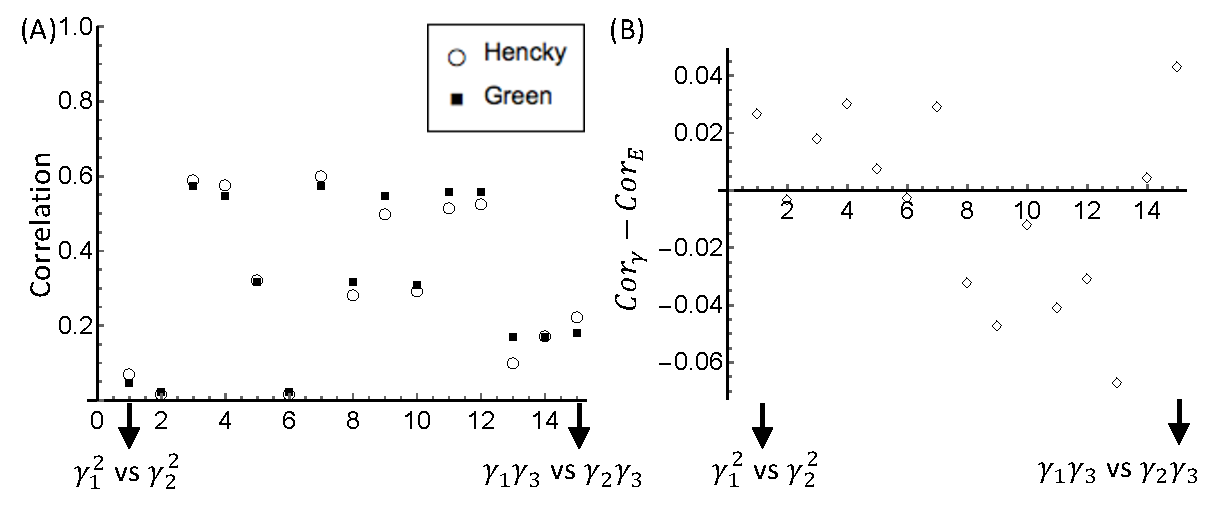
\includegraphics[width=6.5in]{Figures/gvsecorrelation}
\caption{(A) The correlation between parameters pairs in the generalized Fung model when using Green-Lagrange vs Hencky strains. (B) The difference in correlation between each pair of parameters, which is very small but with the Hencky strains being lower overall.}
\label{fig:gvsecorrelation}
\end{figure}
%-------------------	 end FIGURE 	-------------------%
%%%%%%%%%%%%%%%%%%%%%%%%%%%%%%%%%%%%%%%%%%%%%%%%%%%%%%%%%%%%

    
    The last and most important difference between Green-Lagrange and Hencky strains is that they handle compression very differently. Models using Hencky strains tend to increase exponentially under compression, in comparison to models using the Green-Lagrange strains, which only increase mildly with compression. We illustrated this again using the generalized Fung model (Eqn. \ref{eqn:generalizedfungmodel}), with Green-Lagrange or Hencky strain as the input variable (Fig. \ref{fig:gvsecompression}). The reason for this is actually fairly simple, Green-Lagrange strain maps deformations from $\mathbf{E}: [0,\infty] \rightarrow [-1/2,\infty]$, while Hencky strains maps deformations from $\mathbf{\gamma}: [0,\infty] \rightarrow [-\infty,\infty]$, drastically increasing the magnitude of the same strain value under compression. This is problematic, as soft tissues generally behaves very differently under compression than extension. For example, collagen fibers are the most important structural bearing component of most soft tissue. They straighten under extension, which significantly increases the stiffness of the tissue, but buckle and crimp under compression, which does not play a significant role in load bearing \cite{soares_mathematical_2017}. \emph{The behavior of Green-Lagrange strain tensor matches more closely to that of soft tissues}. Due to all factors considered (Table \ref{tb:greenvshencky}), we proceed to use the Green-Lagrange strain tensor as the best kinematic basis to formulate the effective constitutive model. 
    
    
%%%%%%%%%%%%%%%%%%%%%%%%%%%%%%%%%%%%%%%%%%%%%%%%%%%%%%%%%%%%
%-------------------	begin FIGURE 	-------------------%
\begin{figure}
\centering
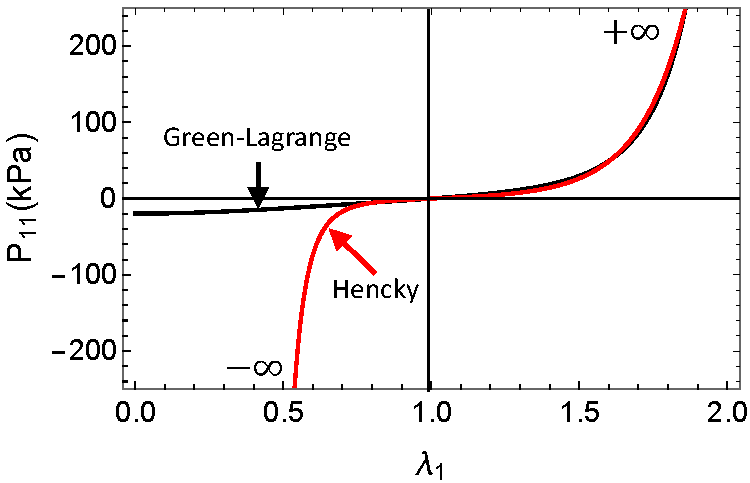
\includegraphics[width=3.25in]{Figures/gvsecompression}
\caption{The response of a generalized Fung model when using Green-Lagrange (Black) vs Hencky strains(Red). Both models are able to match extensional response nearly perfectly with respect to each other, but drastically differ in response under compression.}
\label{fig:gvsecompression}
\end{figure}
%-------------------	 end FIGURE 	-------------------%
%%%%%%%%%%%%%%%%%%%%%%%%%%%%%%%%%%%%%%%%%%%%%%%%%%%%%%%%%%%%


	





%----------------------------------------------------------%
%-------------------	begin TABLE 	-------------------%
\begin{table}
\caption{The difference between using the Green-Lagrange strain tensor versus the Hencky strains to formulate constitutive models. \textbf{Bold} text indicates key advantages and \textit{Italic} text indicate key disadvantages.}
\begin{center}
\label{tb:greenvshencky}
\begin{tabular}{|p{0.9in}|p{2.4in}|p{2.4in}|}
\hline
\rowcolor{Gray}
\multicolumn{1}{|>{\centering\arraybackslash}m{0.9in}|}{Characteristics} 
	& \multicolumn{1}{|>{\centering\arraybackslash}m{2.4in}|}{\textbf{Green-Lagrange strain}} 
    & \multicolumn{1}{|>{\centering\arraybackslash}m{2.4in}|}{\textbf{Hencky strain}}\\
\hline
General & Most commonly used in modeling	& \textbf{Easy to interpret physically} \\
\hline
Stress 	& Even simpler form for the 2nd Piola Kirchhoff stress 
\begin{equation*}
\begin{aligned}
\mathbf{S} =& \dpd{\Psi}{E_m}\mathbf{m}_0\otimes\mathbf{m}_0 + \dpd{\Psi}{E_n}\mathbf{n}_0\otimes\mathbf{n}_0 \\&+ \frac{1}{2}\dpd{\Psi}{E_{\phi}}\left(\mathbf{m}_0\otimes\mathbf{n}_0+\mathbf{n}_0\otimes\mathbf{m}_0\right)
\end{aligned}
\end{equation*}
\normalsize
	& Simple form for the Cauchy stress	%\footnotesize
\begin{equation*}
\begin{aligned}
\mathbf{T} =& \dpd{\Psi}{\gamma_{1}}\mathbf{m}_t\otimes\mathbf{m}_t + \dpd{\Psi}{\gamma_{2}}\mathbf{n}_t\otimes\mathbf{n}_t \\ &+ \frac{\lambda_n}{\lambda_m}\dpd{\Psi}{\gamma_{3}}\left(\mathbf{m}_t\otimes\mathbf{n}_t+\mathbf{n}_t\otimes\mathbf{m}_t\right)
\end{aligned}
\end{equation*}
\normalsize
\\
\hline
\multicolumn{1}{|>{\raggedright}m{0.9in}|}{Elasticity tensor} & \textbf{Much simpler form for the elasticity tensor}
	& \textit{The equations for the elasticity tensor is extremely long} \\
\hline
\multicolumn{1}{|>{\raggedright}m{0.9in}|}{Parameter covariance} 	& 	& \textbf{Modestly less correlation between parameters} \\
\hline
\multicolumn{1}{|>{\raggedright}m{0.9in}|}{Response under compression}	&	\textbf{Modest changes in stress under compression, behaves much more similar to soft tissues due to collagen fiber crimp}
	& \textit{Behaves badly under large compression} \begin{itemize}
	\item Log scaling cause the strain energy to increase exponentially with compression
	\end{itemize}\\
\hline
\end{tabular}
\end{center}
\end{table}
%-------------------	 end TABLE 		-------------------%
%----------------------------------------------------------%

	












